	Une variante de VNM a été proposée par Hernandez et Navarro \citep{hernandez2014compressed}. Comme première contribution, ils augmentent les types de structures découvertes dans la phase de clustering pour englober aussi: les cliques, les bi-cliques. L'extraction de motifs cette fois-ci n'est basée sur un parcours des feuilles vers la racine mais l'inverse où  l'ensemble des sommets finales des liens du motifs est constitués des étiquettes des nœuds de l'arbre inclus dans le chemin de la racine vers la feuille et  les sommets initiales sont la liste des sommets inclus dans le nœud feuille. 
				%%Noublie pas revient vers la source 
				Leurs deuxième contribution consiste en une hybridation dans le but de représenter le graphe en sortie à l'aide de structures compactes. Une première approche proposée est d'utiliser les  k2-trees \citep{brisaboa2009k} et qui donnent la représentation la plus compacte.  
				La deuxième hybridation consiste en une nouvelle structure proposée par les auteur.\\
				%revoire cela avec SAnna
				\begin{figure}[h]
					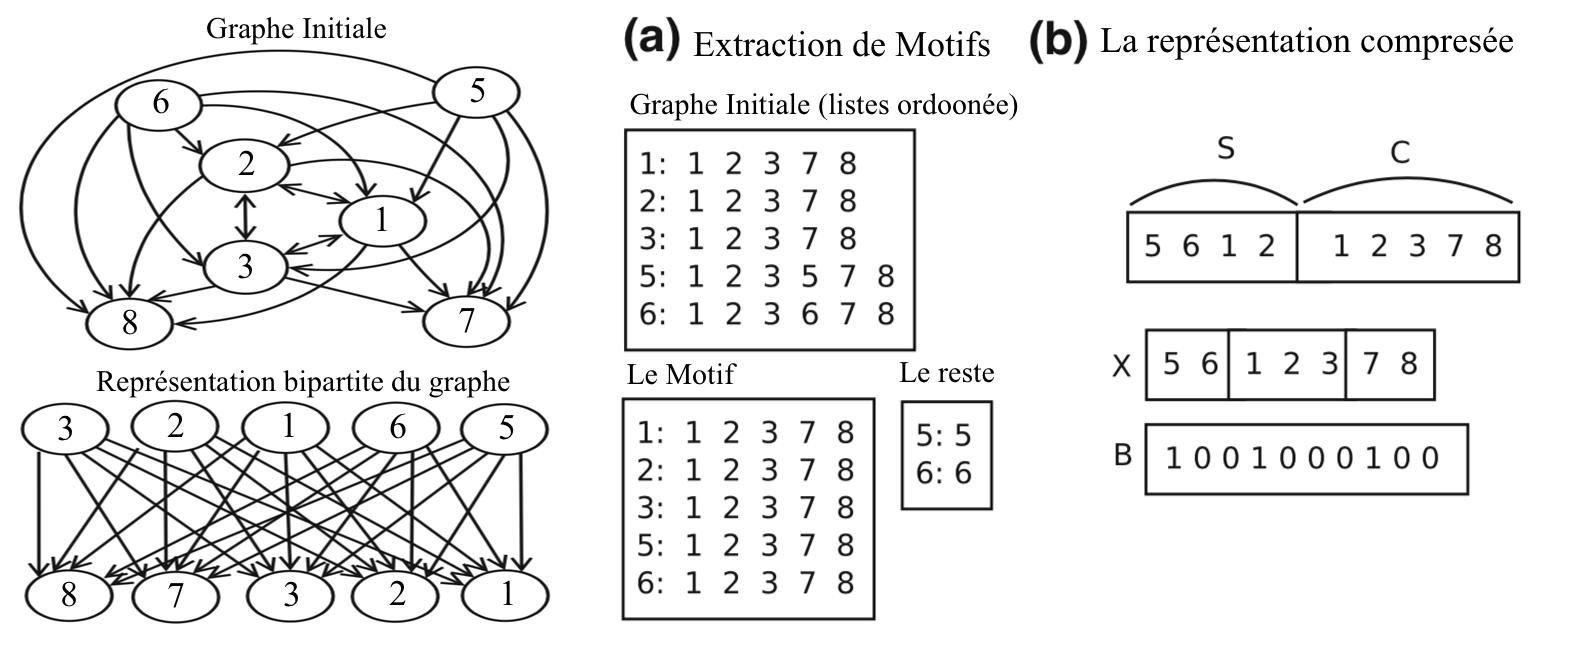
\includegraphics[scale=0.25]{ressources/image/VNM2_exemple.png} 
					\caption{Exemple d'exécution de SDM}
					\label{SDM}
				\end{figure}